% Drift-Aware Adaptive Page Replacement -- LaTeX transcription of the revised manuscript.
% Baseline was a FAITHFUL transcription of the now-removed historical PDF Drift_Aware_Page_Replacement_Revised.pdf; this source is authoritative.
% Fixes are then applied one by one; see CHANGELOG.md.
\documentclass[10pt,twocolumn,a4paper]{IEEEtran}
\usepackage[T1]{fontenc}
\usepackage[utf8]{inputenc}
\usepackage{amsmath,amssymb}
\usepackage{graphicx}
\usepackage{booktabs}
\usepackage{array}
\usepackage{makecell}
\usepackage{xcolor}
\usepackage[hidelinks]{hyperref}
\usepackage{balance}
\usepackage{xr}
\externaldocument{supplement}
\graphicspath{{figs/}}
\setlength{\tabcolsep}{4pt}
\renewcommand{\arraystretch}{1.0}

\begin{document}

\title{When Does Drift Gating Pay Off? A Reproducible Measurement Study of Drift-Aware Page Replacement}

\author{Muhammad~Qasim,~Hunain~Tahir,~Hussain~Ahmad,~and~Mohsin~Ghaffar~Ghouri%
\thanks{M. Qasim, H. Tahir, H. Ahmad, and M. G. Ghouri are with the University
of Management and Technology (UMT), Lahore, Pakistan. M. Qasim is also with the
Anoneurx Research Lab, Anoneurx. Corresponding author: M. Qasim (e-mail:
itskashie@anoneurx.com).}}

\maketitle

\begin{abstract}
When drift-triggered gating pays for adaptive page replacement is unclear. We
report a reproducible measurement study of a CUSUM trigger with sampled
shadow evaluation and a cost-margin switch; an active KS confirmation stage had
small ablation effect and is not a validated gate. On 80 non-stable synthetic
traces, gating saved 76\% of shadow evaluations versus continuous evaluation
(6.47 vs.\ 27.39/trace) but had higher miss ratio (0.453 vs.\ 0.423) and was
not significantly different from S3-FIFO (0.468). On six public FIU block
traces, the frozen controller never switched because of an identified
capacity-sampling fault; a post hoc repair produced identical public,
synthetic, and holdout results. Post hoc follow-ups found a sharp
shadow-rankability boundary ($C_s/D_w<1$) but no meaningful FIU repair gain;
CUSUM dominated periodic/random at matched budgets, while Oracle/ContShadow
exposed an accuracy ceiling; selected Page-Hinkley and simplified ADWIN
detectors did not close the oracle gap. On available real traces and added
SIEVE/W-TinyLFU baselines, DA showed no accuracy advantage. A user-space
minor-fault calibration places the DA--ContShadow crossover at 2.2\,$\mu$s
(95\% CI 1.44--4.06\,$\mu$s), but a total-time envelope that includes CLOCK and
S3-FIFO shows DA is never the cheapest policy on the measured means: CLOCK is
cheapest below 0.216\,$\mu$s, S3-FIFO between 0.216 and 2.305\,$\mu$s, and
continuous evaluation above 2.305\,$\mu$s, with DA at least 3.27\,ns per
reference above the best alternative at every miss cost. Gating reduces shadow
work, but no accuracy advantage was observed in these measurements, and DA is
never best in these measurements.
\end{abstract}

\section{Introduction}
\label{sec:intro}

Physical memory is finite. When a process references a page that is not
resident and no free frame is available, the memory manager must evict a
resident page. The rule that makes this choice, the page-replacement policy,
affects page-fault frequency, storage traffic, tail latency and, ultimately,
application throughput. Recency-based policies such as least recently used
(LRU) and its CLOCK approximation remain the practical default in operating
systems, while the research literature offers frequency-aware, scan-resistant
and self-tuning alternatives, including the adaptive replacement cache (ARC)
[1], CLOCK with adaptive replacement (CAR) [2], the low inter-reference recency
set policy (LIRS) [3], 2Q [4] and S3-FIFO [5].

No single policy is best for every access pattern. A sequential scan can
flush a cache tuned for repeated reuse, a loop slightly larger than memory can
make LRU miss on every reference, and a policy that protects a previously hot
working set can retain pages that are useless after a phase change. Real
workloads move between such regimes: a database alternates between index
lookups and table scans, a scientific code between computation kernels, and a
multitasking system between applications. The question this paper studies is
therefore not which policy is best, but whether a system can recognize that
the reference behaviour has changed and respond at an acceptable cost.

The stakes of this choice have grown. Containerized and multi-tenant servers
interleave unrelated workloads on shared memory, GPU and accelerator memory is
oversubscribed by multitasking and large-model serving, and tiered memory
systems make a wrong eviction more expensive because the next level is slow or
recomputation is costly [26]--[28]. Recent studies show that adaptive and
learned policies can reduce misses substantially [15], [18], [19], but also
that simple policies such as LRU remain surprisingly competitive in some
settings [28] and that policy rankings depend strongly on the workload [29]. A
principled account of when adaptation pays for itself is therefore needed, not
only another adaptive algorithm.

We use workload drift to mean a statistically meaningful change over time in
the distribution or temporal structure of page references. Two research lines
address related problems. Adaptive replacement algorithms infer from feedback
which behaviour to favour: ARC shifts capacity between recency and frequency
lists, LeCaR and CACHEUS reweight expert policies by regret, and recent learned
or learning-augmented designs reduce the cost of learning on the eviction path
[11], [12], [15], [19]. Concept-drift research, in contrast, provides formal
change detectors with controllable error rates, such as adaptive windowing and
sequential tests [6], [7], [20]--[25]. The two lines have overlapping goals
but different constraints. A drift detector built for a machine-learning
pipeline may be too expensive, or rest on assumptions (labels, prediction
errors) that do not exist in a page-reference stream. A replacement algorithm
that adapts continuously may, conversely, switch behaviour without any control
over the rate of unnecessary switches.

A closely related precedent exists outside operating-system paging. Adaptive
cache-mode selection for queries over raw data [34] keeps a shadow cache of the
alternative mode and switches when a significance test favours it. That work
shows that statistically guided cache adaptation is not new; what remains open
is whether drift-gated selection among page-replacement policies is effective
once the costs of monitoring, shadow evaluation and policy-state migration are
counted, and how it compares with strong existing replacement algorithms.

Four constraints make drift-aware replacement hard. (a)~Rate. References
arrive at memory speed, so any per-reference statistical work is prohibitive,
and monitoring must be sampled or summarized by epoch. (b)~Missing labels and
policy-dependent signals. There is no ground truth for ``the workload
changed'', and the most obvious signal, the miss ratio, depends on the active
policy and capacity, so a switch can itself create an apparent change.
(c)~State. Policies keep different metadata, and a switch must rebuild it from
the resident pages; the quality of that migration, and which pages it retains,
can decide whether a switch helps or harms. (d)~Error control. False alarms
waste work and cause oscillation, while missed changes leave a mismatched
policy in place. A design that ignores any of the four can look good on paper
and fail in operation.

This paper makes three contributions. (1)~A controlled measurement of drift
gating against continuous shadow evaluation and strong static baselines, on
freshly generated phase traces, on six public block traces, and on
instrumented real programs with whole programs held out. We report the null
and negative outcomes: the gate is not significantly different from S3-FIFO,
continuous evaluation is more accurate, and on the public traces the gated
policy never switches. (2)~A cost break-even model for the shadow-work saving,
calibrated by a measured user-space minor-fault latency, together with a
total-time envelope over CLOCK, S3-FIFO, ContShadow and DA showing that DA is
never best in these measurements (Section~\ref{sec:breakeven}). (3)~A fully reproducible
negative-result protocol: released simulator, seeds, configurations, per-trace
CSVs, selection sweep, ablations, sensitivity checks, and scripts that
regenerate every table and figure. We do not claim a new replacement algorithm
or a validated statistical gate; the effective mechanism is a CUSUM trigger
with sampled shadow evaluation.

Our research questions are: RQ1 How do recent adaptive replacement policies
detect and respond to changing access behaviour? RQ2 Which drift detectors are
candidates for low-overhead use in memory management? RQ3 What do emerging
GPU, multi-tier and benchmark studies imply for replacement under changing
workloads? RQ4 Can a drift-gated controller with sampled shadow evaluation
select among replacement policies more effectively than fixed and
heuristic-adaptive baselines under controlled phase changes? RQ1--RQ3 are
answered by the review;
RQ4 is answered empirically.

We adopt a deliberately cautious evaluation stance. The protocol fixes the
design and parameters on training traces before test traces are touched,
evaluates all methods on identical traces, uses paired non-parametric
statistics with multiple-comparison correction, includes an offline optimum so
that the remaining gap is visible, and reports negative and null findings. We
also compare against an Acme-style variant that applies the same shadow
evaluation without a drift gate [34], because that comparison isolates what
drift detection itself contributes.

The answer to RQ4 is mixed, and we state it here so that the scope of the
paper is clear. On 80 fresh non-stable generated traces the gated controller
reduced the mean miss ratio by 20.5\% relative to LRU, but was not
significantly different from S3-FIFO (Holm-adjusted $p = 0.09$) and was
significantly worse than continuous shadow evaluation by 0.030 miss ratio. It
cut shadow evaluations by 76\% relative to continuous evaluation, but in this
study not at equal miss ratio. On six public block traces the frozen controller
never switched because of an identified capacity-sampling fault and was
Pareto-dominated by S3-FIFO, a failed external validation; a post hoc repaired
variant selected the same configuration and produced identical public, synthetic, and holdout results. On 15 instrumented programs with whole programs
held out it tied S3-FIFO at higher cost, and no comparison survived Holm
correction. A cost model puts the DA--ContShadow crossover at about $2.2\,\mu$s per miss,
close to the measured minor-fault latency, but including CLOCK and S3-FIFO in
the total-time envelope shows DA is never best in these measurements: CLOCK,
S3-FIFO and ContShadow each occupy part of the lower envelope. We therefore
report where gating saves shadow work, not superiority over existing methods
(Section~V).

The evidence has clear limits. The main experiments use generated traces --
phase traces with known change points and composites of five access models --
not traces collected from running systems. The public block traces are
storage/cache traces rather than virtual-memory paging traces and serve as an
external check only. The Appendix reports a separate, exploratory evaluation
on page traces from 15 instrumented programs with whole programs held out: DA
tied S3-FIFO there, and no comparison survives Holm correction. A faithful
kernel multi-generation LRU (MGLRU) baseline is not possible in page-level
trace replay because the kernel aging and reclaim-pressure signals are absent;
a page-level MGLRU-style abstraction is reported but not claimed as kernel
MGLRU. No production paging traces were collected. Section~V-K reports a
nine-boot QEMU guest-kernel observation with real in-kernel fault-path
durations, but no reclaim function was reached and the cost model still uses a
user-space minor-fault calibration. The simulator measures algorithmic
behaviour and relative cost, not kernel performance. Section~VI and
Section~VII discuss these limitations in detail.

The remainder of the paper is organized as follows. Section~II gives
conceptual background. Section~III states the review scope and synthesizes the
reviewed studies, and Section~IV identifies the research gaps. Section~V
presents the experimental methodology and results. Section~VI discusses
threats to validity, Section~VII the limitations and scope of the claims, and
Section~VIII concludes.

\section{Conceptual Background}
\label{sec:background}

\subsection{Page Replacement and Workload Phases}

A reference trace is an ordered sequence of page identifiers. For a capacity of
$C$ frames, a replacement policy chooses the victim whenever a reference misses
and all frames are occupied. LRU evicts the least recently used page; LFU the
least frequently used; FIFO the oldest; CLOCK approximates LRU with a reference
bit and a circular scan; MRU evicts the most recently used page, which is
favourable for cyclic scans larger than memory. Hybrid designs use several
queues to separate one-time from repeated references [1]--[5]. The miss ratio
is the fraction of references that miss; it is a necessary but incomplete
quality measure, since metadata cost, decision cost and adaptation speed also
matter. Results on storage-block traces are cache-replacement results and are
not direct evidence about virtual-memory paging.

Workload phases differ in working-set size, reuse-distance distribution,
sequentiality and frequency skew. Drift may be abrupt, gradual or recurring
[6]. Phase changes also interact with policy state: a policy that retains
pages of the previous phase (for example MRU, which pins the oldest resident
pages) can perform far worse than its steady-state behaviour suggests until
that state is flushed. This interaction is central to the design and results
of this paper.

\subsection{Workload Drift and Statistical Detection}

Concept-drift research distinguishes changes in the input distribution, in the
input--output relationship, or both [6]. A page-reference stream has no
labels, so a controller must monitor observable summaries such as the miss
ratio or reuse-time distribution. Adaptive windowing (ADWIN) tests whether
sub-windows have different means [7]; Page--Hinkley and CUSUM procedures
accumulate deviations from a reference level and signal when the sum exceeds a
threshold [30]; two-sample tests such as the Kolmogorov--Smirnov (KS) test
compare distributions. Each has assumptions about sample size, independence
and repeated testing that must be addressed in an implementation. Because
memory operations occur at very high rates, a detector for this setting must
avoid per-reference heavy computation and must balance detection delay, false
alarms, memory use and runtime cost.

\subsection{Earlier Adaptive Replacement and Cache Modelling}

SEQ [8] detects long fault sequences and handles them separately, and EELRU
[9] adjusts its eviction point from recency-distribution evidence. ARC [1]
balances recency and frequency using ghost-list hits, CAR [2] transfers the
idea to CLOCK, LIRS [3] uses inter-reference recency, and 2Q [4] separates
newly admitted from re-referenced pages. S3-FIFO [5] shows that FIFO queues
with a small admission queue can match or beat more complex designs. ACME
[10], LeCaR [11] and CACHEUS [12] mix expert policies using regret or learned
feedback; Acme [34] is the closest precedent for statistically guided
switching, but it selects a query-caching mode rather than a page-replacement
policy. For evaluating alternatives cheaply, miniature simulation [13]
emulates a larger cache with a smaller one, and SHARDS [14] estimates
miss-ratio curves from spatially hashed reuse-distance samples; both make
on-demand shadow evaluation feasible, although sampling can distort temporal
structure and policy rankings. On the change-detection side, ADWIN [7] tests
whether sub-windows of an unlabelled stream have different means; it is a
candidate low-cost trigger but has not been evaluated at page-reference rates.
Set dueling in DIP/DRRIP [37] and the multi-generation LRU reclaim path [38]
are positioned in Section~III. These works establish that adaptation,
sampling and change detection each have precedent; the controller studied
here combines them and measures the consequences, and makes no priority claim
for the combination itself.

\section{Review Scope and Approach}
\label{sec:review}

This is a focused narrative review, not a systematic review or meta-analysis.
The study set was selected by the authors to cover adaptive replacement, drift
detection and emerging memory or cache settings, and comprises 15 peer-reviewed
publications and preprints from 2025--2026 plus foundational work needed to
explain the lineage. One study [20] first appeared as a preprint in December
2024 and was published at AAAI 2025. No preregistered search protocol,
duplicate screening or quality scoring was applied, so the review does not
claim systematic completeness, and several included works are preprints.
Results reported in the studies are not pooled or normalized because
workloads, hardware and metrics differ.

The reviewed adaptive and learned policies move learning or control off the
critical path, use re-access feedback, or adapt CLOCK/FIFO-style heuristics;
generic drift detectors offer explicit change evidence but are not evaluated on
page-reference streams at memory-management rates; and GPU, tiered-memory and
benchmark studies show that policy rankings are workload dependent. The closest
precedent is statistical cache-mode selection with shadow entries [34]. Full
per-study descriptions and a dimension-by-dimension comparison are given in the
supplementary material (Tables S.I--S.II).

\section{Previous Research Gaps}
\label{sec:gaps}

The 15 reviewed studies and the closest prior art are summarized in Table~S.I
(supplementary material) by research area, contribution and limitation relative
to low-overhead, drift-aware page replacement. The limitations are framed
against that goal; they are not claims that the original studies fail at their
own objectives, and some are inferred from each study's scope. Reported
results are not recomputed or compared across studies.



Four gaps follow from the reviewed set: detectors are rarely evaluated on
reference streams at the required sampling rates, statistical gating is rarely
compared with heuristic adaptation, transition costs are not reported together
with miss ratio and detection delay, and studies are not directly comparable
across workloads and metrics. Gaps~2--4 are direct observations; Gap~1 is
inferred from the stated scopes of the cited detectors. The full argument,
including the limitations of the narrative review, is in the supplement.

\section{Experimental Methodology and Results}
\label{sec:eval}

\emph{Reproducibility.} Every experimental number in this paper is produced
by released code in the accompanying package: the synthetic trace generator,
all baselines, the controller, the seeds and the raw per-trace output, the
parameter-selection sweep (\texttt{sweep\_selection.py}), the primary-study
driver (\texttt{run\_main\_study.sh}), the table builder
(\texttt{analyze\_main\_study.py}), the appendix interval script
(\texttt{appendix\_intervals.py}), the cost model (\texttt{cost\_model.py}),
the public-trace converter (\texttt{convert\_public\_traces.py}) and the
fault-latency microbenchmark (\texttt{prototype\_fault\_latency.cpp}) are
provided. The selection sweep is run with the released simulator on training
traces (seed 100), and the selected configuration is evaluated once on fresh
traces (seed 5001).

An earlier report of this study used a simulator, seeds and raw output that
were not retained; its tables cannot be regenerated, none of its numbers is
used here, and it is not discussed further.
\begin{figure}[!t]
\centering
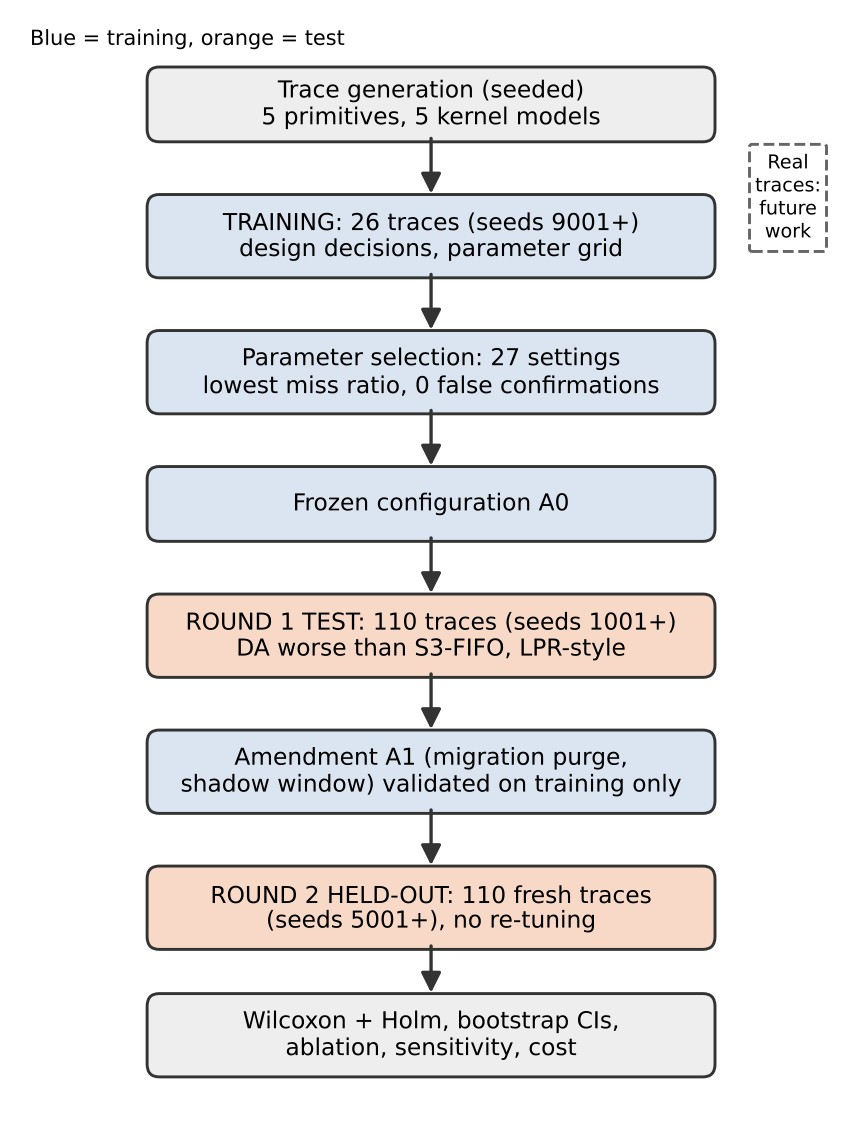
\includegraphics[width=0.85\columnwidth]{fig2_workflow.png}
\caption{Experimental workflow. Blue boxes are training stages, orange boxes
are held-out test rounds.}
\label{fig:workflow}
\end{figure}

\subsection{Simulator, Workloads and Baselines}

We implemented a single-threaded trace-driven simulator in C++ with a capacity
of $C = 1{,}000$ frames, excluding the first 20,000 references (cold fill)
from reported miss ratios. All policies see identical traces. Policies were
sanity-checked against known behaviour: LRU misses on every reference of a
loop larger than memory, and MRU matches the offline optimum on that loop. OPT
minimises misses over the whole trace including the cold fill, so it is a
reference point rather than a strict lower bound on the post-warm-up miss
ratio. Workloads (Table~III) are generated, not
collected: five access primitives with disjoint page ranges, combined into
stable, abrupt, gradual and recurring scenarios with known change points, plus
composite traces from five kernel-level access models (column-wise matrix
traversal, hash join, B-tree lookup, external-sort merge and skewed key-value
lookup with scan bursts). Traces are 110 per round: 30 stable, 20 abrupt,
20 gradual, 20 recurring and 20 composite.

Workloads are generated from five access primitives (LOOP, ZIPF, HOTSCAN,
WINDOW and UNIFORM) combined into stable, abrupt, gradual, recurring and
composite scenarios, plus five kernel-level access models. Eleven baselines
(eight fixed and three adaptive) are compared, with MRU omitted from paired
tests; re-implementations follow the cited descriptions rather than the
authors' code. Definitions, baseline parameters and the two distinct count-
aging rules are listed in the supplement.

The protocol has two stages. (i)~\emph{Training} (seed 100, 15 stable and 32
non-stable traces). A sweep over candidate-set size $\{4,5,6\}$, cost margin
$K \in \{0, 0.05, 0.1, 0.2\}$ and evaluation delay $\{2,5,10,20\}$ selected
five candidates (adding S3-FIFO), $K = 0$, and evaluation delay 10 by the lowest
training miss ratio with zero stable-trace false confirmations. (ii)~\emph{Test}
(fresh seed 5001, 30 stable and 80 non-stable traces), evaluated once with the
frozen configuration. No parameter was changed after the test run. The sweep is
re-executed by \texttt{sweep\_selection.py} with the released simulator on the
same 15+32 training set; the released \texttt{sweep\_results.csv} records every
configuration, and the selected values match the frozen configuration replayed
by \texttt{run\_main\_study.sh}
(\texttt{--ncand 5 --kfrac 0 --z 1.28 --edelay 10}).

\subsection{Controller Under Test}

The controller (Fig.~1) keeps a fast path that serves every reference with the
active policy and updates two counters per page (last access and an aged
count); a sampled subset of references, selected by a 64-bit hash of the page
id with probability $p$, feeds reuse-time and window buffers. All other work
runs once per epoch of $W$ references. The candidate set is
\{LRU, LFU-A, 2Q, MRU, S3-FIFO\}, the five candidates selected on training traces
(Section~V-B); S3-FIFO is therefore inside DA's candidate set, but DA is not
significantly better than S3-FIFO in the reported comparisons. The initial
policy is LRU, and after the first baseline period one shadow evaluation
selects a start policy.

\begin{figure}[!t]
\centering
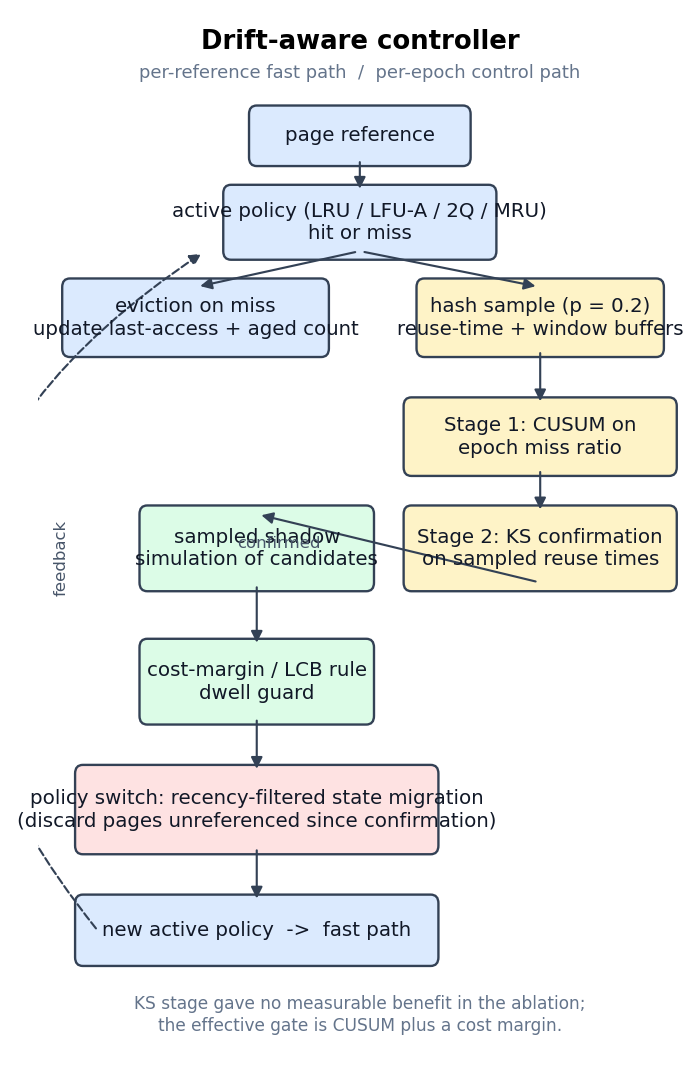
\includegraphics[width=0.85\columnwidth]{fig1_arch.png}
\caption{Architecture of the evaluated controller: per-reference fast path
(blue), per-epoch control path (orange), statistical decision points, and
policy-switching feedback.}
\label{fig:arch}
\end{figure}

\emph{Stage 1.} The epoch miss ratio $m_t$ is standardized as
$z_t = (m_t - \mu_0)/\sigma_0$, with $\mu_0$ and $\sigma_0$ estimated over a
baseline of $B = 8$ epochs ($\sigma_0$ floored at 0.02). A two-sided CUSUM
accumulates
\begin{align}
S_t^{+} &= \max(0,\ S_{t-1}^{+} + z_t - \delta) \label{eq:cusumplus}\\
S_t^{-} &= \max(0,\ S_{t-1}^{-} - z_t - \delta) \label{eq:cusumminus}
\end{align}
and raises an alarm when either statistic exceeds $h$.
\emph{Stage 2.} On an alarm, the sampled reuse times of the last three epochs
(measured in sampled references, with first-time references given a large
sentinel value) are compared with the baseline reuse times by a two-sample KS
test; drift is confirmed if $p < \alpha$ with at least 100 samples per side,
otherwise the alarm is rejected. Because reuse time depends on the workload and
not on the active policy, this stage is intended to separate workload change
from policy-induced miss-ratio change.

\emph{Shadow evaluation.} Ten epochs after confirmation (to accumulate
post-change data), each candidate is simulated at capacity
$C_s = \mathrm{round}(pC)$ on the sampled window starting at the confirmation
epoch. The first 40\% of the window warms the shadow caches, and the remainder
is split into four blocks. For candidate $\pi$, $\Delta_\pi$ is the per-block
miss reduction \emph{per sampled reference} relative to the active policy's
shadow, $B_{\mathrm{raw}}$ the raw references per block, $p$ the sampling rate,
$H$ a fixed horizon and $K = 0.1C$ a transition-cost margin in miss-equivalents.
Dividing by $p$ rescales sampled misses to raw references, so the controller
switches to the candidate with the largest margin if
\begin{equation}
\bigl(\mathrm{LCB}(\Delta_\pi) / (p\,B_{\mathrm{raw}})\bigr) H - K > 0
\label{eq:switch}
\end{equation}
where LCB is a one-sided lower confidence bound ($z = 1.28$) across the four
blocks. The frozen configuration sets $K = 0$, so the margin term did not
constrain the reported switches. A reverse switch to the previous policy within 30 epochs must
additionally exceed $K$ (hysteresis), and a dwell time of 10 epochs applies
after any switch. Switching rebuilds the target policy's metadata from the
resident pages ordered by last access, after discarding pages not referenced
in the last 20,000 references (A1); LFU-A and 2Q use the aged counts to place
pages. After a confirmed change the controller re-baselines for $4 + 10$ epochs
plus $B$ epochs. Table~V lists all parameters. The persistence safeguard of the
design (several consecutive confirmed epochs) was not implemented; the
monitored features were the miss ratio (Stage 1) and sampled reuse times
(Stage 2) only.

The frozen configuration fixes capacity, epoch length, sampling rate, CUSUM
and KS parameters, evaluation delay, shadow capacity, confidence bound, dwell
and migration rules after training; the full parameter table is in the
supplement. The effective mechanism remains a CUSUM trigger with sampled shadow
evaluation, not a validated two-stage gate.

\subsection{Metrics and Statistical Analysis}

The primary metric is the miss ratio after warm-up, reported with the
percentage reduction relative to LRU. Detection is evaluated on all 80
non-stable traces across four scenarios (abrupt, gradual, recurring and
composite; 380 true boundaries in total, which is what the 278/380 figure
denominates): a boundary is detected if a confirmed alarm occurs within
30,000 references after it, and the delay is the distance to that alarm. A
confirmed alarm outside every such window is counted as spurious. On stable
traces confirmations are counted both over the whole trace and after reference
100,000, the latter excluding an initial transient. A reversal is a switch
A$\to$B$\to$A within 60,000 references. Cost is the simulated wall-clock time per reference of the single
released simulator on this machine; it is indicative, not a kernel measurement.
Recovery time, memory overhead and full ranking agreement were not measured in
this reproducible study.

The unit of analysis is the trace (80 non-stable, 30 stable). For every
comparison in this paper the primary uncertainty statement is the percentile
interval over traces (10,000 resamples for means, 5,000 for paired
differences); paired differences are also tested with the Wilcoxon signed-rank
test [33] and Holm correction [35] across the ten baseline comparisons, and
effect sizes are mean and median paired differences with win/loss counts.
Traces in one scenario share a generator, so they are not independent draws
from a population of real workloads; only five access primitives and five
kernel models underlie all traces, and the effective number of independent
units is smaller than 80. The trace-level intervals are therefore conditional
on this design. A four-cluster resampling check is reported only as a coarse sensitivity
note in the supplement; the trace-level paired interval remains the primary
uncertainty statement.

\subsection{Replacement Quality}

All numbers in this section come from the frozen configuration and the fresh
test traces; the raw per-trace CSV output is in the reproduction package.
Table~VI and Figs.~3--5 give the primary result. On the 80 non-stable traces
the controller's mean miss ratio was 0.453 (95\% CI 0.423--0.484), 20.5\%
below LRU (0.570). The offline optimum reached 0.302. The controller was
better than S3-FIFO (0.468) on the mean, but the paired difference was not
significant (Holm-adjusted $p = 0.09$; Table~VII). It was significantly
\emph{worse} than continuous shadow evaluation (ContShadow, 0.423) by 0.030
miss ratio (adjusted $p < 0.001$). On the 30 stable traces the controller
scored 0.307, close to ContShadow (0.307) and better than S3-FIFO (0.330) and
LRU (0.519), largely because of start-up policy selection.

\emph{Stable-trace gain is not drift-handling gain.} A stable trace contains no
phase change, so a benefit there cannot be attributed to drift detection. On
the 30 stable traces DA scored 0.3071 with 0.80 switches and 1.73 shadow
evaluations per trace, against LRU 0.5186, S3-FIFO 0.3301 and ContShadow
0.3065. That advantage over LRU comes from the initial shadow evaluation that
chooses a start policy and from continued re-evaluation, not from responding
to drift. The drift-handling comparison is the non-stable result above, where
DA is 0.030 worse than ContShadow despite saving 76\% of shadow work. We do
not add the stable-trace gain to the drift-handling claim.

By scenario the controller is close to ContShadow on abrupt and recurring
traces but clearly behind it on gradual drift and composite traces; the
scenario-level numbers are retained verbatim in the supplement.

\begin{table}[!t]
\caption{Mean Miss Ratio by Scenario and Overall (Fresh Test Traces)}
\label{tab:quality}
\footnotesize
\setlength{\tabcolsep}{2pt}
\begin{tabular}{@{}lccccc@{}}
\toprule
Method & Abrupt & Gradual & Recurring & Composite & Non-stable \\
\midrule
LRU & 0.500 & 0.572 & 0.527 & 0.682 & 0.570 [0.540, 0.598] \\
FIFO & 0.536 & 0.609 & 0.560 & 0.696 & 0.600 [0.573, 0.627] \\
CLOCK & 0.487 & 0.558 & 0.515 & 0.677 & 0.559 [0.530, 0.589] \\
LFU-A & 0.474 & 0.535 & 0.505 & 0.671 & 0.546 [0.515, 0.576] \\
MRU & 0.943 & 0.928 & 0.902 & 0.968 & 0.935 [0.918, 0.949] \\
2Q & 0.457 & 0.504 & 0.479 & 0.648 & 0.522 [0.493, 0.551] \\
ARC & 0.465 & 0.520 & 0.496 & 0.634 & 0.529 [0.499, 0.557] \\
S3-FIFO & 0.406 & 0.441 & 0.412 & 0.615 & 0.468 [0.435, 0.501] \\
LeCaR & 0.476 & 0.545 & 0.503 & 0.680 & 0.551 [0.520, 0.582] \\
LPR-style & 0.477 & 0.535 & 0.474 & 0.646 & 0.533 [0.509, 0.556] \\
ContShadow & 0.365 & 0.401 & 0.384 & 0.541 & \textbf{0.423} [0.400, 0.446] \\
DA & 0.370 & 0.439 & 0.398 & 0.604 & \textbf{0.453} [0.423, 0.484] \\
OPT & 0.244 & 0.269 & 0.242 & 0.452 & 0.302 [0.281, 0.324] \\
\bottomrule
\end{tabular}
\end{table}

\begin{figure}[!t]
\centering
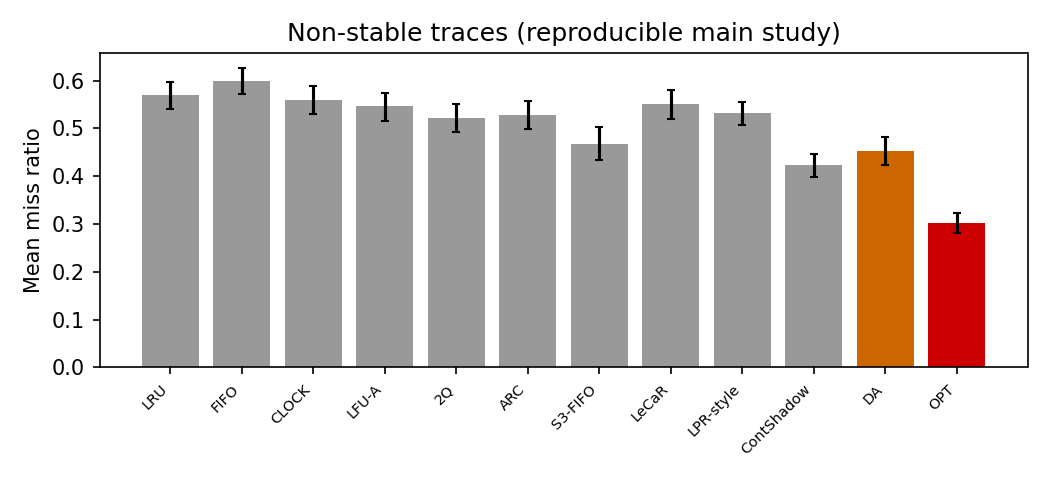
\includegraphics[width=0.85\columnwidth]{fig3_overall.png}
\caption{Mean miss ratio on the 80 non-stable traces with 95\% bootstrap
intervals (reproducible main study, $C = 1{,}000$).}
\label{fig:overall}
\end{figure}

\begin{figure}[!t]
\centering
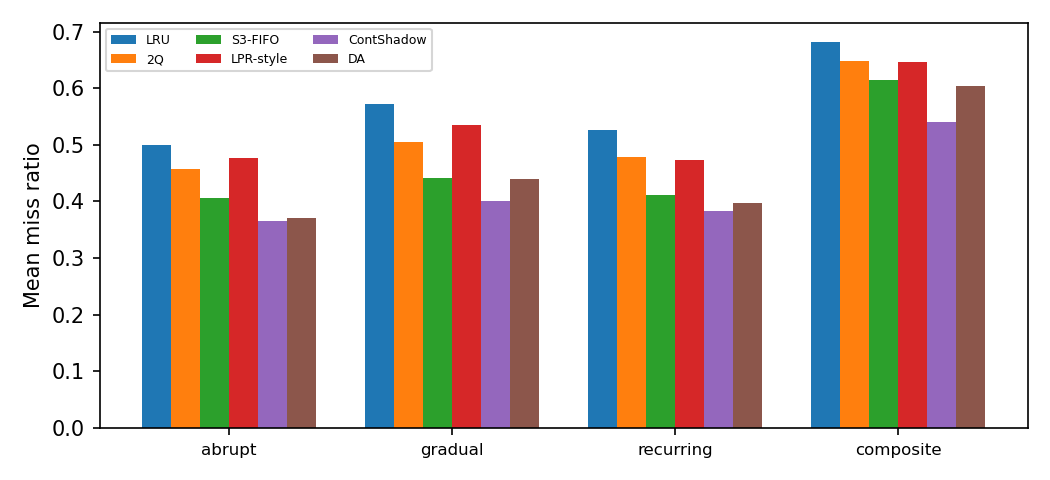
\includegraphics[width=0.85\columnwidth]{fig4_scenario.png}
\caption{Mean miss ratio by scenario on the fresh test traces.}
\label{fig:scenario}
\end{figure}

The paired table (mean differences, bootstrap intervals, win/loss/tie counts
and Holm-adjusted $p$-values for ten baselines) is moved to the supplement;
its interpretation is summarised below.

The paired comparisons reported in the supplement show that negative
differences favour the controller. It was significantly better than eight of the ten baselines after
Holm correction (all adjusted $p < 0.001$). The exception was S3-FIFO, where
the mean favoured DA by only 0.015 and the adjusted $p$ was 0.09: the evidence
for an improvement over the strongest fixed policy is therefore weak. The
other exception is unfavourable: ContShadow had a 0.030 lower mean miss ratio
(adjusted $p < 0.001$), so continuous shadow evaluation was more accurate than
drift-gated evaluation in this study. The paired differences are shown in the supplement.
Bootstrap intervals describe uncertainty in the mean; the Wilcoxon test uses
ranks, so the two need not agree. Intervals are not corrected for multiplicity
or for clustering of traces by scenario.

The post hoc capacity-sampling repair re-selected the same configuration and
gave identical synthetic-trace results; the full paragraph is in the
supplement.

\begin{figure}[!t]
\centering
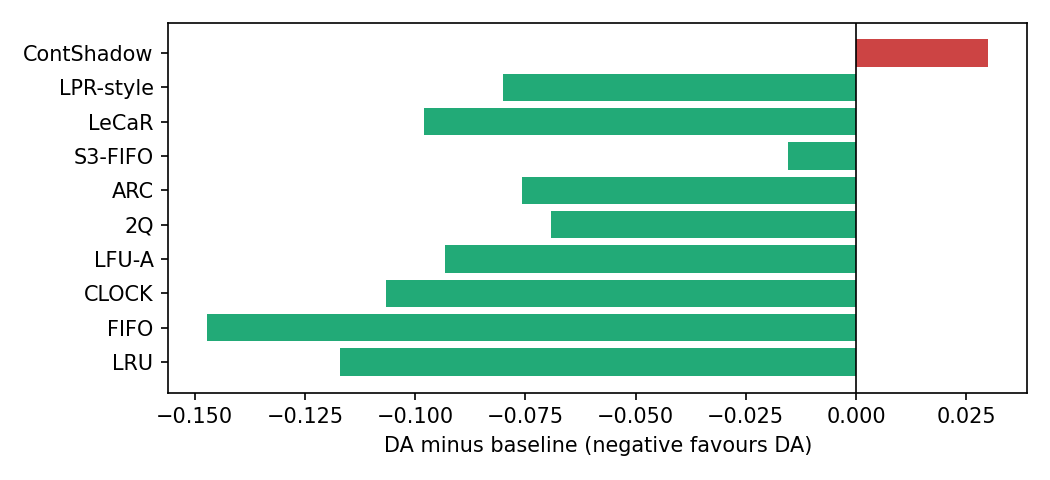
\includegraphics[width=0.85\columnwidth]{fig5_paired.png}
\caption{Paired differences in miss ratio between DA and each baseline on the
80 non-stable traces (negative favours DA).}
\label{fig:paired}
\end{figure}

\subsection{Ablation}

Ablation confirms that shadow evaluation is the essential component:
replacing it with a random choice raises the non-stable miss ratio from 0.453
to 0.619. The other variants lie in 0.453--0.456; the KS stage was active on
all 643 alarms but had a small miss-ratio effect, while the cost margin and
dwell rule were inactive in the frozen run ($K=0$, zero dwell blocks).
S3-FIFO is cheaper (28.5\,ns/reference) but less accurate (0.468), whereas
ContShadow is more accurate (0.423) at 133.4\,ns/reference with 27.39 rather
than 6.47 shadow evaluations per trace. The ablation table, activation counts
and figure are in the supplement.

\subsection{Detection, Switching and Cost}

The trigger detected 278/380 phase boundaries (73.2\%) with a median delay of
2,000 references; detection was strong on abrupt and recurring changes and
weak on gradual changes (24/100). Boundary alignment favours detection, and
the offset sensitivity (274--281 detected, 169--173 spurious confirmations)
is detailed in the supplement.

Simulated time per reference was 25.1 ns for LRU, 8.9 for CLOCK, 28.5 for
S3-FIFO, 36.8 for 2Q, 50.2 for LPR-style, 67.4 for DA and 133.4 for
ContShadow: DA cost 2.7 times LRU and 2.4 times S3-FIFO. These are relative
figures from an unoptimized single-threaded simulator, not kernel latency. DA
is slower and, in this study, less accurate than ContShadow, but cheaper;
against S3-FIFO it is both slower and (non-significantly) more accurate. No
configuration here beat the best static policy on both cost and quality.

Simulated time per reference was 25.1\,ns for LRU, 8.9 for CLOCK, 28.5 for
S3-FIFO, 36.8 for 2Q, 50.2 for LPR-style, 67.4 for DA and 133.4 for
ContShadow: DA cost 2.7 times LRU and 2.4 times S3-FIFO. These are relative
figures from an unoptimized single-threaded simulator, not kernel latency; DA
is slower and less accurate than ContShadow but cheaper, and no configuration
beat the best static policy on both cost and quality. The cost--quality figure
is in the supplement.

\subsection{Post Hoc Measurement Experiments}
\label{sec:posthoc}
The measurements below were run after the frozen main-study results were
obtained. They are reported as post hoc measurements, not as primary
claims or as selected configurations. Raw outputs are in
\texttt{reproduction/trigger\_real/}, \texttt{reproduction/param\_sweep/},
and \texttt{reproduction/rankability\_real/}; commands, seeds, and defaults
are recorded in \texttt{NOT\_DONE.md}.

Post hoc trigger variants, FIU trigger checks, one-at-a-time parameter sweeps
and capacity/sampling rankability sweeps are reported in the supplement; the
summary table below retains the representative outcomes. These measurements
are post hoc and are not used as selected configurations or primary claims.

\subsection{Public Block-Trace Check}
\label{sec:public}
Six FIU web/block traces from the CMU PDL collection [39] were replayed with
the frozen controller configuration and seed 5001. The public traces are
storage block/cache traces rather than virtual-memory paging traces; the
conversion, independent capacity pilot and exact commands are in the supplement.

\begin{table}[!t]
\caption{Public FIU Block Traces: Means Over Six Traces (Raw Output
\texttt{public\_trace\_results.csv})}
\label{tab:public}
\footnotesize
\setlength{\tabcolsep}{4pt}
\begin{tabular}{@{}lccc@{}}
\toprule
Method & Mean miss ratio & Mean ns/ref & Mean shadow evals \\
\midrule
OPT & 0.4595 & 0.0 & 0.00 \\
S3-FIFO & 0.5772 & 31.7 & 0.00 \\
2Q & 0.6209 & 38.3 & 0.00 \\
ARC & 0.6580 & 37.0 & 0.00 \\
LRU & 0.6753 & 25.5 & 0.00 \\
DA & 0.6753 & 82.5 & 13.50 \\
ContShadow & 0.6753 & 180.1 & 48.33 \\
FIFO & 0.6808 & 17.6 & 0.00 \\
\bottomrule
\end{tabular}
\end{table}

Table~\ref{tab:public} reports the means. DA, ContShadow and LRU have the same
miss ratio on every one of the six traces (mean 0.6753), and DA made zero
switches on every trace, with 11--15 KS-confirmed alarms per trace and no true
boundaries. S3-FIFO had both a lower mean miss ratio (0.5772) and a lower mean
simulated time (31.7 versus 82.5 ns/reference), so DA is \emph{Pareto-dominated}
by S3-FIFO on this trace set; DA is also weakly dominated by LRU, which matches
its miss ratio at 25.5 ns/reference. Gating saved 72\% of the shadow
evaluations of continuous evaluation here but yielded no accuracy gain.

Diagnostics found a capacity--sampling fault: at $C=20{,}000$ the shadow
capacity $C_s=4{,}000$ exceeded the roughly 1,100--1,800 distinct pages in each
sampled window, so all candidates incurred only compulsory misses and tied.
The post hoc identity cap ($f=1.0$) did not restore rankability or change the
zero-switch, no-gain outcome. Per-trace maxima, margins, re-selection and
repair details are in the supplement.

These are storage block/cache traces, not virtual-memory page traces, and only
a prefix of each was replayed; this is an external check and not the primary
evidence for paging.

\subsection{Post Hoc Follow-up Measurements}
\label{sec:posthoc_followups}

The following measurements are recorded in \texttt{PROTOCOL.md}
(first committed to git on 2026-11-24; no independent pre-run timestamp
exists) and are reported as post hoc. They test repairs and
alternatives suggested by the negative main result; null and negative
outcomes are reported.

\begin{table}[!t]
\caption{Post hoc follow-ups: outcome and representative numbers. Details
and raw-table pointers are in Section S4 of the supplementary material.}
\label{tab:prespec}
\footnotesize
\setlength{\tabcolsep}{3pt}
\begin{tabular}{@{}p{0.18\columnwidth}p{0.74\columnwidth}@{}}
\toprule
Follow-up & Outcome (key numbers) \\
\midrule
Phase 1 rankability & $C_s/D_w\ge1$ gives 0/1514 rankable evals; no FIU repair gain (C=20000 test 0.6621). \\
Phase 2 budget frontier & CUSUM better than periodic/random near 6.2--7.0 evals; Oracle 0.4335, ContShadow 0.4228 accuracy ceiling. \\
Phase 3 detectors & PH 0.4552, ADWIN 0.4991 vs CUSUM 0.4529; neither closes oracle gap. \\
Phase 4 baselines/traces & SIEVE 0.5557, W-TinyLFU 0.4913, LHD 0.6736 synth; real-trace DA no advantage; PDL FIU originals: S3-FIFO 0.6188 best, DA 0.6280. \\
Phase 5 robustness & 2.2\,$\mu$s DA/ContShadow crossover is calibration only; t3 LCB DA 0.4586 vs 0.4529 (negative); DA never on total-time envelope. \\
\bottomrule
\end{tabular}
\end{table}

\subsection{Additional measured checks: six PDL families and asynchronous shadow evaluation}
\label{sec:additional}
We replayed six 1M-reference prefixes from the CMU PDL collection at 18 family$\times$capacity points. Across those points the mean miss ratios were S3-FIFO 0.4683, ContShadow 0.4739, DA 0.4742, CLOCK 0.4973 and LRU 0.4987 (Table~\ref{tab:pdl_main}); the paired DA$-$S3-FIFO difference was $+0.0059$ with Holm $p=0.0192$, so \textbf{DA is worse than S3-FIFO on the measured means}.
\begin{table}[t]
\caption{Phase 6: selected methods across six CMU PDL families (18 points)}
\label{tab:pdl_main}
\centering\footnotesize
\begin{tabular}{@{}lccc@{}}
\toprule
Method & Mean miss & Shadow evals/trace & ns/ref \\
\midrule
CLOCK & 0.4973 & 0.00 & 9.5 \\
LRU & 0.4987 & 0.00 & 41.0 \\
S3-FIFO & 0.4683 & 0.00 & 43.4 \\
DA & 0.4742 & 2.67 & 94.4 \\
ContShadow & 0.4739 & 13.11 & 147.5 \\
\bottomrule
\end{tabular}
\end{table}

A real user-space asynchronous shadow worker on the 80 non-stable traces gave mean miss ratios 0.5611, 0.5676 and 0.5599 in three repetitions, with paired async$-$sync differences $+0.1082$, $+0.1147$ and $+0.1070$ (Table~\ref{tab:async_main}). Across 240 timing rows there were 15,066 stale decisions, 1,192 applied results and 0 dropped. This is a \textbf{negative result}: asynchronous execution is clearly worse than synchronous DA in these measurements.
\begin{table}[t]
\caption{Phase 7: real asynchronous-shadow prototype, 80 non-stable traces per repetition}
\label{tab:async_main}
\centering\footnotesize
\begin{tabular}{@{}lccc@{}}
\toprule
Rep. & Mean miss & DA$-\!$sync [95\% CI] & Win/Tie/Loss \\
\midrule
1 & 0.5611 & $+0.1082$ [$+0.0726$,$+0.1471$] & 12/0/68 \\
2 & 0.5676 & $+0.1147$ [$+0.0793$,$+0.1537$] & 9/0/71 \\
3 & 0.5599 & $+0.1070$ [$+0.0743$,$+0.1430$] & 8/0/72 \\
\bottomrule
\end{tabular}
\end{table}

\subsection{QEMU guest-kernel observation}
A post hoc Linux 6.6.1 QEMU guest replayed three conditions in three fresh boots each: fixed LRU (\texttt{lru\_gen/enabled=0x0000}), fixed MGLRU (\texttt{0x0007}) and a user-space CUSUM controller coupled to the same sysfs knob. Function-graph tracing was restricted to five recorded fault/reclaim functions present in the guest; 191,370 durations were parsed. Table~\ref{tab:kernel_main} reports the measured fault-path durations and vmstat deltas. The observation is null: all nine runs show 131,138 minor faults, zero \texttt{workingset\_refault\_anon}, zero \texttt{pgscan\_anon}/\texttt{pgsteal\_anon} deltas, and zero controller toggles. Only \texttt{handle\_mm\_fault} and \texttt{do\_wp\_page} produced samples; no reclaim function was reached. The captured cgroup \texttt{memory.max}/\texttt{memory.peak} files were empty, so memory pressure was not demonstrated. These are real in-kernel fault-path timings under an MGLRU-enabled guest, not a kernel DA policy or a reclaim-latency result.
\begin{table}[t]
\caption{Phase 8: real guest-kernel observations; ftrace row is handle\_mm\_fault}
\label{tab:kernel_main}
\centering\footnotesize
\setlength{\tabcolsep}{2pt}
\begin{tabular}{@{}lcccc@{}}
\toprule
Condition & Minor faults & Refaults & Toggles & Median/p95 fault ns \\
\midrule
fixed\_lru & 131,138 & 0 & 0 & $761.0/1593.0$ \\
fixed\_lru & 131,138 & 0 & 0 & $671.0/1522.0$ \\
fixed\_lru & 131,138 & 0 & 0 & $752.0/1643.9$ \\
fixed\_mglru & 131,138 & 0 & 0 & $641.0/1532.0$ \\
fixed\_mglru & 131,138 & 0 & 0 & $711.5/1573.0$ \\
fixed\_mglru & 131,138 & 0 & 0 & $741.0/1643.0$ \\
coupled & 131,138 & 0 & 0 & $731.0/1673.0$ \\
coupled & 131,138 & 0 & 0 & $741.0/1693.0$ \\
coupled & 131,138 & 0 & 0 & $701.0/1583.0$ \\
\bottomrule
\end{tabular}
\end{table}


\subsection{Cost Break-Even and Total-Time Envelope}
\label{sec:breakeven}

Using the measured means (DA 0.453 versus ContShadow 0.423 miss ratio, 6.47
versus 27.39 shadow evaluations per trace), the cost model gives a DA--
ContShadow crossover of 2.2\,$\mu$s per miss (95\% CI 1.44--4.06\,$\mu$s)
calibrated by a user-space minor-fault measurement. Across CLOCK, S3-FIFO,
ContShadow and DA, \textbf{DA is never the cheapest policy on the measured
means}: CLOCK, S3-FIFO and ContShadow each occupy part of the lower envelope.
The full derivation, bootstrap intervals and calibration detail are in the
supplement.

\begin{table*}[t]
\caption{Total time per reference by miss cost, using the measured per-reference times and mean miss ratios of the 80 non-stable test traces. Panel (a): bold marks the lowest total in each row; DA is never the lowest, and the last column gives its excess over the best policy. Panel (b): pairwise crossing miss costs; the DA/S3-FIFO interval is unstable because the miss-ratio difference is small. All values are point estimates; bootstrap intervals are in the text.}
\label{tab:breakeven}
\centering\footnotesize
\setlength{\tabcolsep}{3pt}
\textbf{(a) Total time per reference ($\mu$s)}
\par\vspace{2pt}
\begin{tabular}{@{}lccccccc@{}}
\toprule
Miss-cost scenario & $c_m$ ($\mu$s) & CLOCK & S3-FIFO & ContShadow & DA & Cheapest & DA$-$best (ns) \\
\midrule
DRAM (illustrative) & 0.1 & \textbf{0.065} & 0.075 & 0.176 & 0.113 & CLOCK & 47.8 \\
CLOCK/S3-FIFO crossing & 0.215539 & \textbf{0.129} & \textbf{0.129} & 0.224 & 0.165 & CLOCK/S3-FIFO & 35.5 \\
Minor-fault calibration (measured) & 2.2 & 1.240 & \textbf{1.059} & 1.064 & 1.064 & S3-FIFO & 4.9 \\
S3-FIFO/ContShadow crossing & 2.304942 & 1.298 & \textbf{1.108} & \textbf{1.108} & 1.111 & S3-FIFO/ContShadow & 3.3 \\
Remote/RDMA (illustrative low) & 5 & 2.806 & 2.370 & \textbf{2.248} & 2.332 & ContShadow & 84.3 \\
Remote/RDMA (illustrative high) & 10 & 5.603 & 4.712 & \textbf{4.362} & 4.596 & ContShadow & 234.5 \\
NVMe SSD (illustrative low) & 20 & 11.197 & 9.395 & \textbf{8.590} & 9.125 & ContShadow & 535.1 \\
NVMe SSD (illustrative high) & 100 & 55.950 & 46.860 & \textbf{42.417} & 45.356 & ContShadow & 2939.5 \\
Swap/page fault (illustrative) & 1000 & 559.417 & 468.339 & \textbf{422.966} & 452.955 & ContShadow & 29989.5 \\
\bottomrule
\end{tabular}
\par\vspace{4pt}
\textbf{(b) Pairwise crossing miss costs ($\mu$s)}
\par\vspace{2pt}
\begin{tabular}{@{}lcc@{}}
\toprule
Pair & Crossing & 95\% CI \\
\midrule
CLOCK / S3-FIFO & 0.216 & [0.171, 0.274] \\
S3-FIFO / ContShadow & 2.305 & [1.660, 3.678] \\
DA / ContShadow & 2.196 & [1.449, 4.105] \\
DA / S3-FIFO & 2.517 & [1.086, 22.051] \\
\bottomrule
\end{tabular}
\par\smallskip
\footnotesize DA/S3-FIFO interval uses 9394/10{,}000 positive bootstrap replicates. Minimum DA excess over the best policy: 3.27\,ns/ref [-28.6, 40.2] at $c_m\approx2.30\,\mu$s; the interval includes zero, so the crossing is not statistically resolved.
\end{table*}


The minor-fault calibration, illustrative miss-penalty rows and the
analytical asynchronous-shadow variant are described in the supplement; they
do not turn gating into an accuracy advantage.

\begin{figure}[!t]
\centering
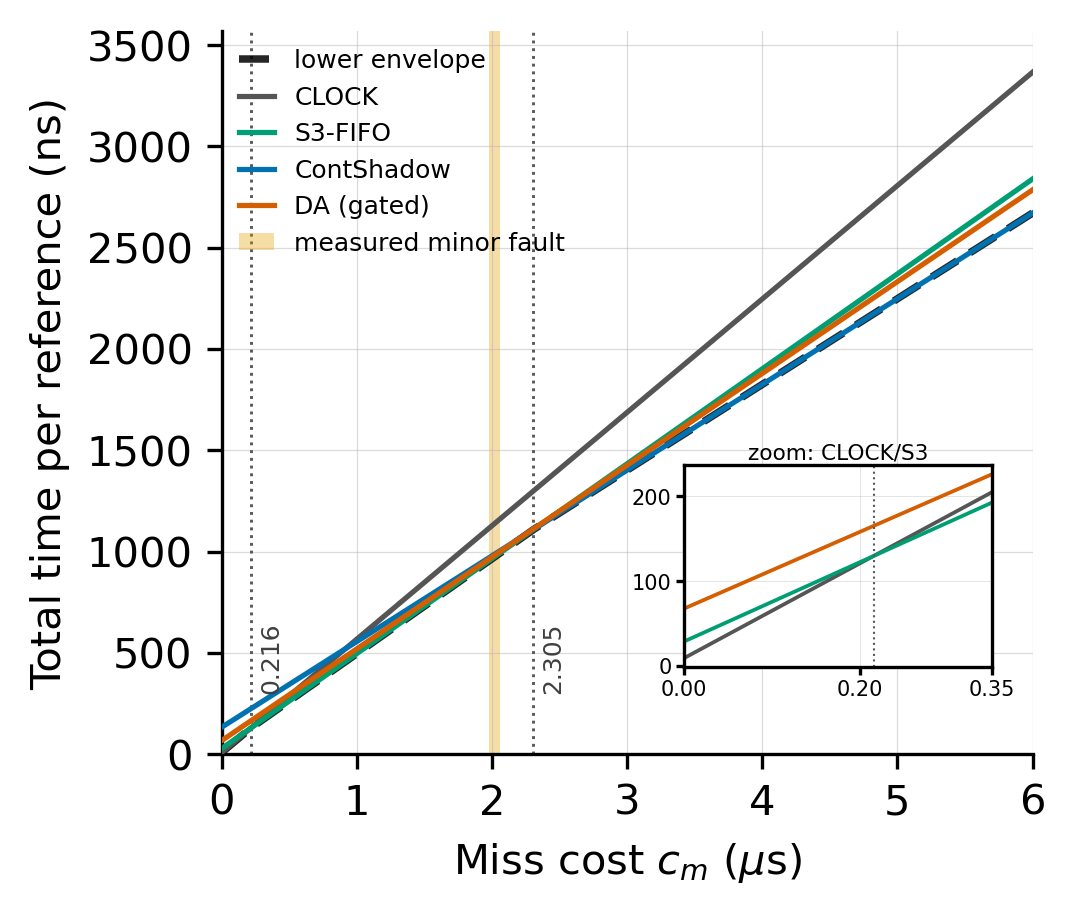
\includegraphics[width=0.85\columnwidth]{fig8_breakeven.png}
\caption{Total time per reference versus miss cost for CLOCK, S3-FIFO,
ContShadow and DA, with the lower envelope of the three comparators (black
dashed). CLOCK is cheapest below 0.216\,$\mu$s, S3-FIFO between 0.216 and
2.305\,$\mu$s, and ContShadow above 2.305\,$\mu$s; DA is never on the envelope,
with a minimum excess of 3.27\,ns/reference at 2.305\,$\mu$s. The orange band
is the measured minor-fault cost; the inset zooms the CLOCK/S3-FIFO crossing.}
\label{fig:breakeven}
\end{figure}

\subsection{Capacity Sensitivity}

At $C=500$ the controller scored 0.580 against LRU 0.693 and S3-FIFO 0.590,
but was again behind ContShadow (0.555); the table is in the supplement.

\subsection{Hypothesis Outcomes}

We frame three hypotheses. H1: the drift-aware controller attains a lower miss
ratio than the strongest fixed baseline (S3-FIFO). H2: a two-stage gate (CUSUM
trigger plus KS confirmation) improves miss ratio and detection over a single
CUSUM trigger with the same sampled shadow evaluation; the frozen run used the
design margin $K = 0$. H3: the controller's simulated per-reference cost remains
competitive with fixed and adaptive baselines. A previously listed hypothesis
about sampled shadow evaluation ranking candidates consistently with
full-capacity evaluation was dropped because full ranking agreement was not
measured; no claim is made from it.
Table~\ref{tab:hypotheses} reports the outcomes. No cost budget or agreement
threshold was specified before the study; post hoc criteria are not treated as
prospectively registered results.

\begin{table}[!t]
\caption{Hypothesis Outcomes (Reproducible Main Study)}
\label{tab:hypotheses}
\footnotesize
\begin{tabular}{@{}p{0.06\columnwidth}p{0.30\columnwidth}p{0.56\columnwidth}@{}}
\toprule
 & Outcome & Evidence \\
\midrule
H1 & Not supported & DA 0.453 vs S3-FIFO 0.468 ($-0.015$, adjusted $p = 0.09$); better than LRU and seven other baselines. \\
H2 & Not supported & ContShadow had lower miss ratio; the KS stage was active on all 643 alarms but had a small miss-ratio effect (0.456 without KS vs.\ 0.453 with KS); detection rate 73.2\%. \\
H3 & Not met & $2.7\times$ LRU per reference; DA is never on the lower total-time envelope (minimum excess 3.27\,ns/ref at $c_m\approx2.30\,\mu$s). \\
\bottomrule
\end{tabular}
\end{table}

The design lessons are narrow: shadow evaluation is the component that
matters, and gating saves shadow work at a miss-ratio cost here rather than
delivering an accuracy advantage. The expanded lesson-by-lesson discussion is
in the supplement.

\section{Threats to Validity}
\label{sec:threats}

Threats include generated traces with epoch-aligned changes, re-implemented
baselines, simulator-only costs, a normal quantile applied to four correlated
shadow blocks, and traces clustered by generator; the KS stage had a small
miss-ratio effect (0.456 without KS versus 0.453 with KS) despite being active
on all 643 alarms. The full construct, internal, external and statistical
threats discussion is in the supplement.

\section{Limitations and Scope of Claims}
\label{sec:limits}

The study is a trace-driven simulation of one controller on generated,
public block and exploratory program traces, with no claim of superiority over
strong replacement policies. A nine-boot QEMU guest observation measured real
in-kernel fault-path durations, but produced no reclaim event, no controller
toggle and no reclaim-latency result, and no in-kernel DA replacement policy
was built. Full limitations, including the non-faithful MGLRU-style
abstraction and the reviewed real-trace follow-ups, are in the supplement.

\section{Conclusion}
\label{sec:conclusion}

This paper asks when drift gating pays off in page replacement and answers it
as a reproducible measurement study. The evidence includes the frozen main
study, post hoc diagnostics, and post hoc follow-ups: a CUSUM-triggered
controller with sampled shadow evaluation is compared against continuous
shadow evaluation, static baselines, trigger alternatives, PH/ADWIN detectors,
and SIEVE/W-TinyLFU baselines; a cost break-even model is calibrated by a
user-space minor-fault measurement; and code, seeds, outputs, and protocols are
released.

On 80 non-stable synthetic traces, gating saved 76\% of shadow evaluations
but had higher miss ratio than continuous evaluation (0.453 vs.\ 0.423) and
was not significantly different from S3-FIFO (Holm-adjusted $p=0.09$). The FIU
capacity-sampling fault remained a failed external validation after repair.
Post hoc follow-ups showed a sharp rankability boundary without a
meaningful FIU repair gain, CUSUM budget-frontier advantage over
periodic/random but not over oracle/ContShadow accuracy, and no oracle-gap
closure by selected PH/ADWIN. On available real traces with SIEVE/W-TinyLFU,
DA showed no accuracy advantage. The 2.2\,$\mu$s minor-fault calibration and
illustrative miss-cost/async variants locate the DA--ContShadow crossover, but
the total-time envelope shows DA is never best in these measurements: CLOCK,
S3-FIFO and ContShadow each occupy part of the lower envelope and DA remains
at least 3.27\,ns/reference above the best alternative. External FIU originals
from [39] reproduced the absence of a DA advantage; stronger claims require the
remaining production traces and kernel-level measurements.

\section*{Appendix: Exploratory Real-Program Evidence}
\addcontentsline{toc}{section}{Appendix: Exploratory Real-Program Evidence}

The exploratory fifteen-program whole-program holdout found DA 0.3304 against
S3-FIFO 0.3291 and LRU 0.3540, with no Holm-significant comparison (smallest
adjusted $p=0.096$). Detailed methods, kernels, paired intervals and cost
figures are in the supplement.

\section*{Declarations}
\addcontentsline{toc}{section}{Declarations}

\emph{Data and code availability.} The simulator, trace generators, seeds,
configuration files, raw per-trace output and analysis scripts for the
reproducible main study are released in the accompanying
\texttt{reproduction/} package. \texttt{sweep\_selection.py} regenerates the
parameter-selection sweep, \texttt{run\_main\_study.sh} regenerates every
primary table and figure, \texttt{appendix\_intervals.py} regenerates the
appendix percentile intervals, and \texttt{cost\_model.py} together with
\texttt{prototype\_fault\_latency.cpp} regenerates the break-even analysis, and
\texttt{phase5/total\_time\_envelope.py} regenerates the total-time table,
figure and envelope.
The public-trace converter, the public-trace result and detection CSVs, the
independent capacity-pilot CSVs, and the boundary-offset detection CSVs are included in the
same package; the source traces are available from the repository in [39].
The instrumented programs and raw output for the exploratory real-program
appendix are included in the same package. The QEMU guest-kernel build,
workload and controller sources, raw traces and derived CSVs are included in
\texttt{phase8\_kernel/}; no in-kernel DA replacement prototype was built.

\emph{Funding.} This research was conducted independently without external
financial funding.

\emph{Conflict of interest.} M. Qasim is affiliated with both the University of
Management and Technology (UMT), Lahore, and Anoneurx Research Lab, Anoneurx;
the corresponding-author e-mail is at Anoneurx. The other authors are
affiliated with UMT. Anoneurx Astra, a tool developed at Anoneurx, was used for
prose drafting and code/analysis assistance, as disclosed below. Anoneurx
provided no funding for this work and had no role in study design, data
collection, analysis, interpretation or publication. No other competing
financial or non-financial interests are declared.

\emph{Use of AI-assisted tools.} AI-assisted tools, including Anoneurx Astra
and ChatGPT, were used to help draft and edit prose and to assist with code
development and analysis scripts. All experimental results were produced and
verified by the authors with the released code, and the authors take full
responsibility for the content of the paper.

\begin{thebibliography}{39}

\bibitem{r1} N. Megiddo and D. S. Modha, ``ARC: A self-tuning, low overhead
replacement cache,'' in \emph{Proc. 2nd USENIX Conf. File Storage Technol.
(FAST)}, 2003, pp. 115--130.

\bibitem{r2} S. Bansal and D. S. Modha, ``CAR: Clock with adaptive
replacement,'' in \emph{Proc. 3rd USENIX Conf. File Storage Technol. (FAST)},
2004, pp. 187--200.

\bibitem{r3} S. Jiang and X. Zhang, ``LIRS: An efficient low inter-reference
recency set replacement policy to improve buffer cache performance,'' in
\emph{Proc. ACM SIGMETRICS}, 2002, pp. 31--42.

\bibitem{r4} T. Johnson and D. Shasha, ``2Q: A low overhead high performance
buffer management replacement algorithm,'' in \emph{Proc. 20th Int. Conf. Very
Large Data Bases (VLDB)}, 1994, pp. 439--450.

\bibitem{r5} J. Yang, Y. Zhang, Z. Qiu, Y. Yue, and K. V. Rashmi, ``FIFO
queues are all you need for cache eviction,'' in \emph{Proc. 29th ACM Symp.
Oper. Syst. Princ. (SOSP)}, 2023, pp. 130--149.

\bibitem{r6} J. Gama, I. \v{Z}liobait\.{e}, A. Bifet, M. Pechenizkiy, and A.
Bouchachia, ``A survey on concept drift adaptation,'' \emph{ACM Comput.
Surv.}, vol. 46, no. 4, Art. no. 44, 2014.

\bibitem{r7} A. Bifet and R. Gavald\`a, ``Learning from time-changing data
with adaptive windowing,'' in \emph{Proc. SIAM Int. Conf. Data Mining (SDM)},
2007, pp. 443--448.

\bibitem{r8} G. Glass and P. Cao, ``Adaptive page replacement based on memory
reference behavior,'' in \emph{Proc. ACM SIGMETRICS}, 1997, pp. 115--126.

\bibitem{r9} Y. Smaragdakis, S. Kaplan, and P. Wilson, ``EELRU: Simple and
effective adaptive page replacement,'' in \emph{Proc. ACM SIGMETRICS}, 1999,
pp. 122--133.

\bibitem{r10} I. Ari, A. Amer, R. Gramacy, E. L. Miller, S. A. Brandt, and D.
D. E. Long, ``ACME: Adaptive caching using multiple experts,'' in \emph{Proc.
Workshop Distrib. Data Struct. (WDAS)}, 2002.

\bibitem{r11} K. Vietri \emph{et al.}, ``Driving cache replacement with
ML-based LeCaR,'' in \emph{Proc. 10th USENIX Workshop Hot Topics Storage File
Syst. (HotStorage)}, 2018.

\bibitem{r12} L. V. Rodriguez \emph{et al.}, ``Learning cache replacement
with CACHEUS,'' in \emph{Proc. 19th USENIX Conf. File Storage Technol. (FAST)},
2021, pp. 341--354.

\bibitem{r13} C. Waldspurger, T. Saemundsson, I. Ahmad, and N. Park, ``Cache
modeling and optimization using miniature simulations,'' in \emph{Proc. USENIX
Annu. Tech. Conf. (ATC)}, 2017, pp. 487--498.

\bibitem{r14} C. A. Waldspurger, N. Park, A. Garthwaite, and I. Ahmad,
``Efficient MRC construction with SHARDS,'' in \emph{Proc. 13th USENIX Conf.
File Storage Technol. (FAST)}, 2015, pp. 95--110.

\bibitem{r15} W. Zhou, Z. Niu, Y. Xiong, J. Fang, and Q. Wang, ``3L-Cache:
Low overhead and precise learning-based eviction policy for caches,'' in
\emph{Proc. 23rd USENIX Conf. File Storage Technol. (FAST)}, 2025, pp.
237--254.

\bibitem{r16} H. Kim, ``Learning-based page replacement scheme for efficient
I/O processing,'' \emph{Sci. Rep.}, vol. 15, 2025, doi:
10.1038/s41598-025-88736-4.

\bibitem{r17} G. Yuan, X. Li, S. Wu, Y. Zhu, D. Yang, C. Yao, X. Tang, and G.
Chen, ``EACLOCK: An efficient and adaptive page replacement algorithm to
understand your workload,'' \emph{IEEE Trans. Knowl. Data Eng.}, vol. 38,
no. 11, pp. 7387--7401, Nov. 2026, doi: 10.1109/TKDE.2026.3724159.
\url{https://doi.org/10.1109/TKDE.2026.3724159}.

\bibitem{r18} Y. Zhai \emph{et al.}, ``Clock2Q+: A simple and efficient
replacement algorithm for metadata cache in VMware vSAN,'' \emph{Proc. VLDB
Endow.}, vol. 19, no. 12, pp. 3874--3887, 2026, doi: 10.14778/3827998.3828002.

\bibitem{r19} H. Xia, W. Nixon, B. D. Marthen, P. Bhandari, and J. Yang,
``Learning-augmented heuristics: Simple yet smart, robust and interpretable
cache eviction,'' in \emph{Proc. 20th USENIX Symp. Oper. Syst. Design Implement.
(OSDI)}, 2026, pp. 2241--2259.

\bibitem{r20} P. Lu, J. Lu, A. Liu, and G. Zhang, ``Early concept drift
detection via prediction uncertainty,'' in \emph{Proc. AAAI Conf. Artif.
Intell.}, 2025; arXiv:2412.11158.

\bibitem{r21} N. Tan, Y.-C. Shih, D. Yang, and A. Salunkhe, ``Flexible and
efficient drift detection without labels,'' arXiv:2506.08734, 2025.

\bibitem{r22} P. Lu, J. Lu, A. Liu, E. Yu, and G. Zhang, ``Autonomous concept
drift threshold determination,'' arXiv:2511.09953, 2025.

\bibitem{r23} N. Harshit and K. Mounvik, ``Improving real-time concept drift
detection using a hybrid transformer-autoencoder framework,''
arXiv:2508.07085, 2025.

\bibitem{r24} S. Bandyopadhyay, J. Bose, and S. Roy Chowdhury, ``A hybrid
framework for real-time data drift and anomaly identification using
hierarchical temporal memory and statistical tests,'' \emph{Int. J. Math. Eng.
Manag. Sci.}, vol. 10, no. 3, pp. 777--796, 2025, doi:
10.33889/ijmems.2025.10.3.039.

\bibitem{r25} D. N. Assis and V. M. A. Souza, ``ADWIN-U: Adaptive windowing
for unsupervised drift detection on data streams,'' \emph{Knowl. Inf. Syst.},
2025, doi: 10.1007/s10115-025-02523-1.

\bibitem{r26} W. Shen, Y. Chen, R. Chen, and H. Chen, ``Towards fully-fledged
GPU multitasking via proactive memory scheduling,'' arXiv:2512.24637, 2025.

\bibitem{r27} Y. Zheng \emph{et al.}, ``gpu\_ext: Extensible OS policies for
GPUs via eBPF,'' arXiv:2512.12615, 2025.

\bibitem{r28} Y. Liu, M. Yu, and J. Yang, ``When fancy eviction fails:
Rethinking cache replacement for LLM prefix reuse,'' arXiv:2609.28870, 2026,
doi: 10.48550/arXiv.2609.28870.

\bibitem{r29} N. Patel and H. Maniar, ``Comparative evaluation of cache
replacement algorithms for time-bounded stale-tolerant data workloads,''
\emph{Int. J. Sci. Res. Technol.}, vol. 3, no. 6, pp. 556--564, 2026, doi:
10.5281/zenodo.20576370. \url{https://doi.org/10.5281/zenodo.20576370};
\url{https://ijsrtjournal.com/article/comparative-evaluation-of-cache-replacement-algorithms-for-time-bounded-stale-tolerant-data-workloads}.

\bibitem{r30} E. S. Page, ``Continuous inspection schemes,'' \emph{Biometrika},
vol. 41, no. 1--2, pp. 100--115, 1954.

\bibitem{r31} D. Narayanan, A. Donnelly, and A. Rowstron, ``Write
off-loading: Practical power management for enterprise storage,'' \emph{ACM
Trans. Storage}, vol. 4, no. 3, Art. no. 10, 2008.

\bibitem{r32} L. A. Belady, ``A study of replacement algorithms for a
virtual-storage computer,'' \emph{IBM Syst. J.}, vol. 5, no. 2, pp. 78--101,
1966.

\bibitem{r33} F. Wilcoxon, ``Individual comparisons by ranking methods,''
\emph{Biometrics Bull.}, vol. 1, no. 6, pp. 80--83, 1945.

\bibitem{r34} T. Azim, A. Nadeem, and A. Ailamaki, ``Adaptive cache mode
selection for queries over raw data,'' in \emph{Proc. 9th Int. Workshop
Accelerating Analytics Data Manag. Syst. Using Modern Processor Storage Archit.
(ADMS@VLDB)}, 2018, pp. 51--65.

\bibitem{r35} S. Holm, ``A simple sequentially rejective multiple test
procedure,'' \emph{Scand. J. Stat.}, vol. 6, no. 2, pp. 65--70, 1979.

\bibitem{r36} S. Jiang, F. Chen, and X. Zhang, ``CLOCK-Pro: An effective
improvement of the CLOCK replacement,'' in \emph{Proc. USENIX Annu. Tech. Conf.
(ATC)}, 2005, pp. 323--336.

\bibitem{r37} M. K. Qureshi, A. Jaleel, Y. N. Patt, S. C. Steely Jr., and J.
Emer, ``Adaptive insertion policies for high performance caching,'' in
\emph{Proc. 34th Int. Symp. Comput. Archit. (ISCA)}, 2007, pp. 381--391, doi:
10.1145/1250662.1250709.

\bibitem{r38} Linux Kernel Organization, ``Multi-gen LRU,'' Linux kernel
documentation, 2026. [Online]. Available:
\url{https://docs.kernel.org/mm/multigen_lru.html}

\bibitem{r39} CMU Parallel Data Laboratory, ``Cache eviction tactics:
cacheDatasets trace collection,'' online data repository and format README,
accessed Nov. 24, 2026. The project page links to the \texttt{cacheDatasets}
repository; its FIU directory contains
\texttt{fiu\_madmax-110108-112108.oracleGeneral.zst}. The README specifies
zstd-compressed 24-byte request records and citation requirements, but no
dataset-specific licence; PDL's site-wide copyright notice says materials
distributed by the server are provided on a non-commercial basis. [Online].
Available: \url{https://pdl.cmu.edu/CacheEviction/index.shtml};
\url{https://ftp.pdl.cmu.edu/pub/datasets/twemcacheWorkload/cacheDatasets/};
\url{https://ftp.pdl.cmu.edu/pub/datasets/twemcacheWorkload/cacheDatasets/README};
\url{https://pdl.cmu.edu/Publications/copyright.shtml}.

\end{thebibliography}

\end{document}
